% ------------------------------------------------------------------
%  B4卒業論文
%  December, 2023
%  by Hiroyuki Ohno
%  Last Update : 
% ------------------------------------------------------------------
\documentclass[a4paper,twocolumn,9pt]{jsarticle}
\usepackage{amsmath}
\usepackage[dvipdfmx]{graphicx}
\usepackage{tutAbstract}
\usepackage[hang,small,bf]{caption}
\usepackage[subrefformat=parens]{subcaption}

\Title{不整地生成AIを用いたロボットの未知環境適応のための\\実験フレームワークに関する研究1}		%タイトル
\StudentNumber{201809}			%学籍番号
\Name{大野\ 裕之}									% 氏名
\Teacher{垣内\ 洋平}								% 指導教員名
% アブストラクト({の次に改行する場合,%を付けないと空白が入ります.)
% 改行を使いたい場合は\\でお願いします.
% 段落を使いたい場合,1行開けはエラーになってしまうので,\\と\IndentEngを使ってください.
\AbstractText{%											
This paper describes an experimental framework for robot exploration of uneven terrain environments using generative AI.
While robots are expected to be used in unknown environments, it is difficult for robots to adapt to such environments and successfully explore them.
One way to solve this problem is to use machine learning to plan a run, but there is a limit to the amount of training terrain data that can be prepared for this purpose.
In this paper, we propose an experimental framework that uses GAN as generative AI to generate unknown rough terrain to secure a huge amount of learning data and improve the robot's running performance.
We also evaluate the effectiveness of the generated terrain by comparing the trajectory of the robot when it runs on the original and generated terrain data, respectively.
}

\begin{document}
%タイトル
\TitleText

%本文
\section{はじめに}
近年では,災害現場や月面などの未知環境におけるロボットの活用が,人の活動領域の拡大やその際に起こりうる人の身の危険性を回避するという点で期待されている.しかし,それら未知の環境に対してロボットが自動操作のみで探査を行うのは困難である.また,その走行計画で機械学習を用いる場合、地形データを収集するのにも限界がある.そこで本研究では,ロボットが走行する未知の不整地環境を効率的に生成する方法と,その地形を評価するための走行実験フレームワークを提案する.

\section{地形データの収集方法}
% \subsection{本研究で想定する未知環境}
対象にする未知環境は,危険性等の理由でロボットの自動制御による探査が求められる環境であることと,そのデータ収集がロボットに対して地形の特性上困難であることの二つを考慮する.これに従い,本研究では未知環境の例として月面を取り扱う.

% \subsection{地形生成によるデータ収集}
月面データの収集方法について,生成AIモデルであるGAN(Generative Adversarial Network)をボクセルベースに応用した3D-GAN\cite{bunken1}を用いた.NASAが提供している25種類の月面メッシュファイル(図\ref{fig:moon_nasa})を学習用データセットとし,ボクセルに変換した後その三次元分布からGANによって新たなボクセルデータを生成する[図\ref{fig:moon_voxel}].最終的にそのボクセルデータを再度メッシュ化することで不整地データを作成する[図\ref{fig:moon_gen}].

%図
\begin{figure}[b]
  \centering
  \begin{minipage}[b]{0.4\linewidth}
    \centering
    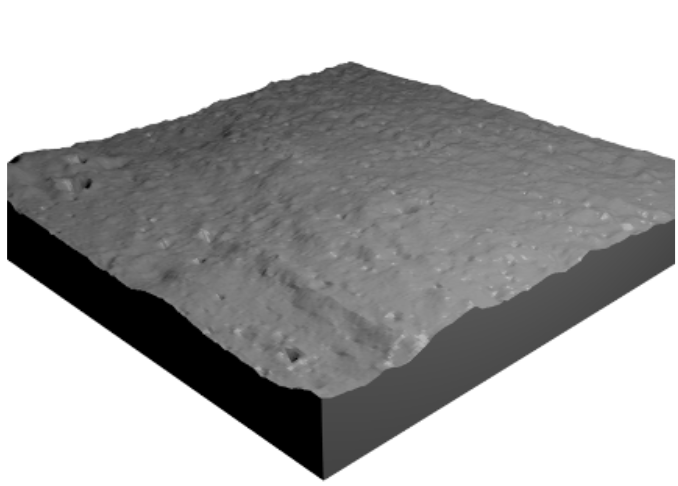
\includegraphics[keepaspectratio, scale=0.1]{figures/NASA_moon.png}
    \subcaption{NASAの月面データ}\label{fig:moon_nasa}
  \end{minipage}
  \begin{minipage}[b]{0.4\linewidth}
    \centering
    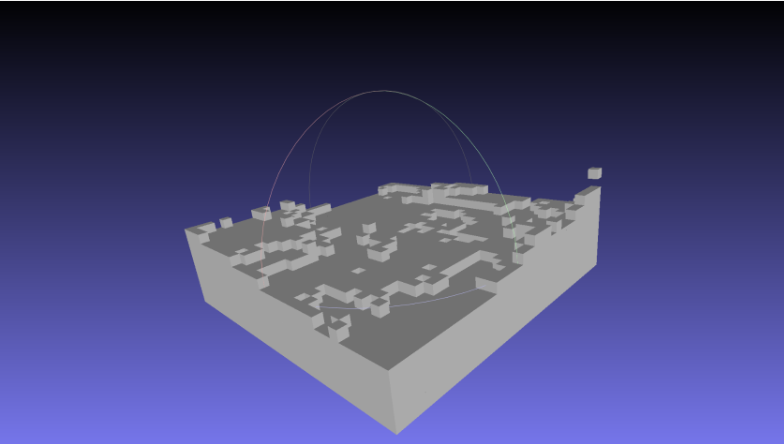
\includegraphics[keepaspectratio, scale=0.1]{figures/moon_voxel.png}
    \subcaption{ボクセル化した月面データ}\label{fig:moon_voxel}
  \end{minipage}
  \begin{minipage}[b]{0.4\linewidth}
    \centering
    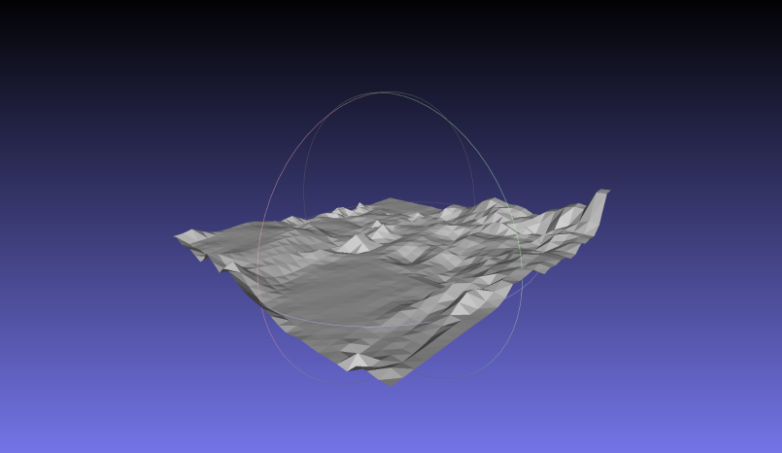
\includegraphics[keepaspectratio, scale=0.1]{figures/moon_mesh.png}
    \subcaption{生成した月面データ}\label{fig:moon_gen}
  \end{minipage}
  \begin{minipage}[b]{0.4\linewidth}
    \centering
    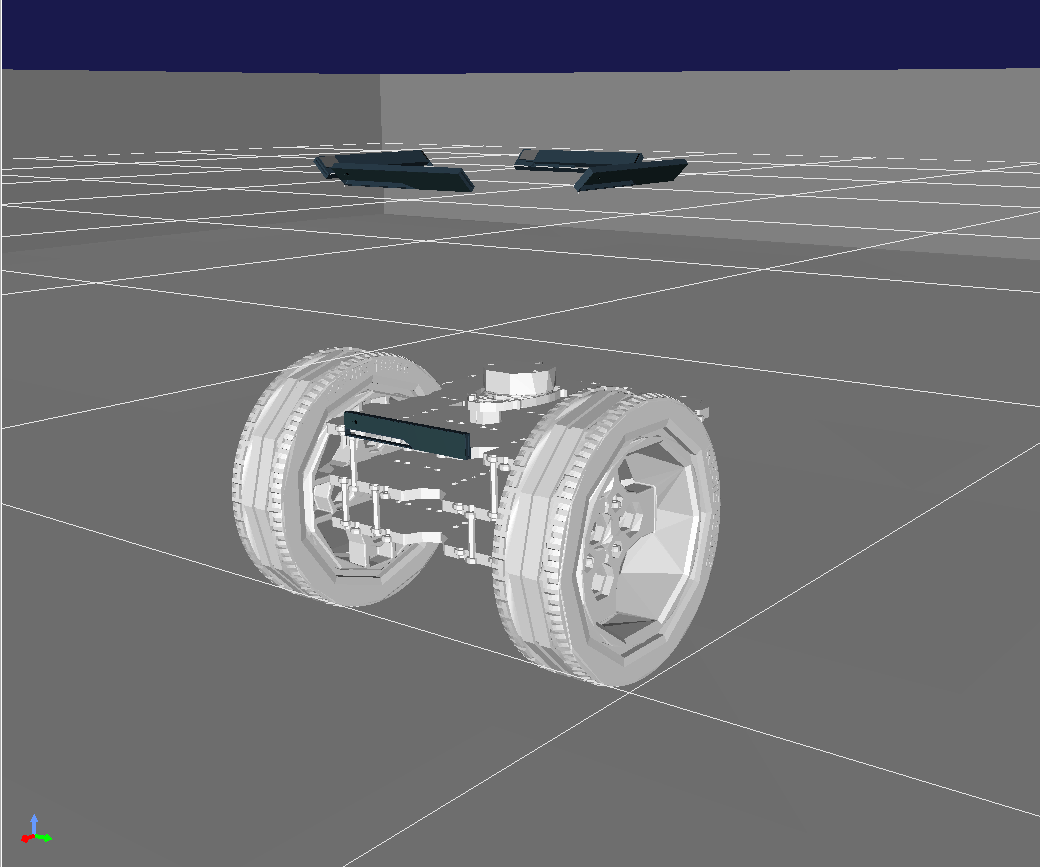
\includegraphics[keepaspectratio, scale=0.07]{figures/robot_visual.png}
    \subcaption{使用したロボット}\label{fig:robot}
   \end{minipage}
  \caption{月面データの生成}
\end{figure}

\section{使用するロボットの構成と走行計画手法}
\subsection{ロボットの構成}
使用するロボットには,外界のセンシング機能と不整地に対する一定の走破性能を持ったハードウェアがそれぞれ要求される.そこで使用するロボットには,図\ref{fig:robot}のような径の大きな2つのタイヤと2つのキャスタ,深度カメラを4方向に向け搭載した.


 \subsection{走行計画手法}
走行計画として,4つの深度カメラから得られた画像から走行可能な方位を選択する方法を用いた.事前に生成した地形を用いて走行実験を行い,ある方位に走行可能だった場合はsafeとして0,転倒や脱輪により探査続行不可になった場合はその直前の画像にdangerとして1をラベリングする.そのデータに対し出力が0から1になるよう機械学習し,走行中に推論した結果最も0に近い値を出力した方位に向かうようにした.

\section{実験方法}
予め生成した複数の不整地上を手動操作でロボットに走行させ,機械学習用データを収集する。学習モデルにはCNN(Convolutional Neural Network)を使用した.上記のデータを用いて学習を行い,再度生成した不整地上をロボットに走行させながらその軌跡を保存する.走行するマップ範囲内での軌跡の含有率をロボットの走破性とした\cite{bunken2}.シミュレーションにはロボット用統合GUIソフトウェアであるchoreonoidを用いた.


\section{生成地形の評価}
上記の学習済みモデルを用いて,生成した不整地上と元の月面上をそれぞれ2分間走行させた際の軌跡に対し,マップの走破性を比較することで生成地形の有用性を評価した.結果は図\ref{fig:result1},図\ref{fig:result2}のようになった.

\begin{figure}[b]
  \centering
  % \begin{minipage}[b]{0.45\linewidth}
  %   \centering
  %   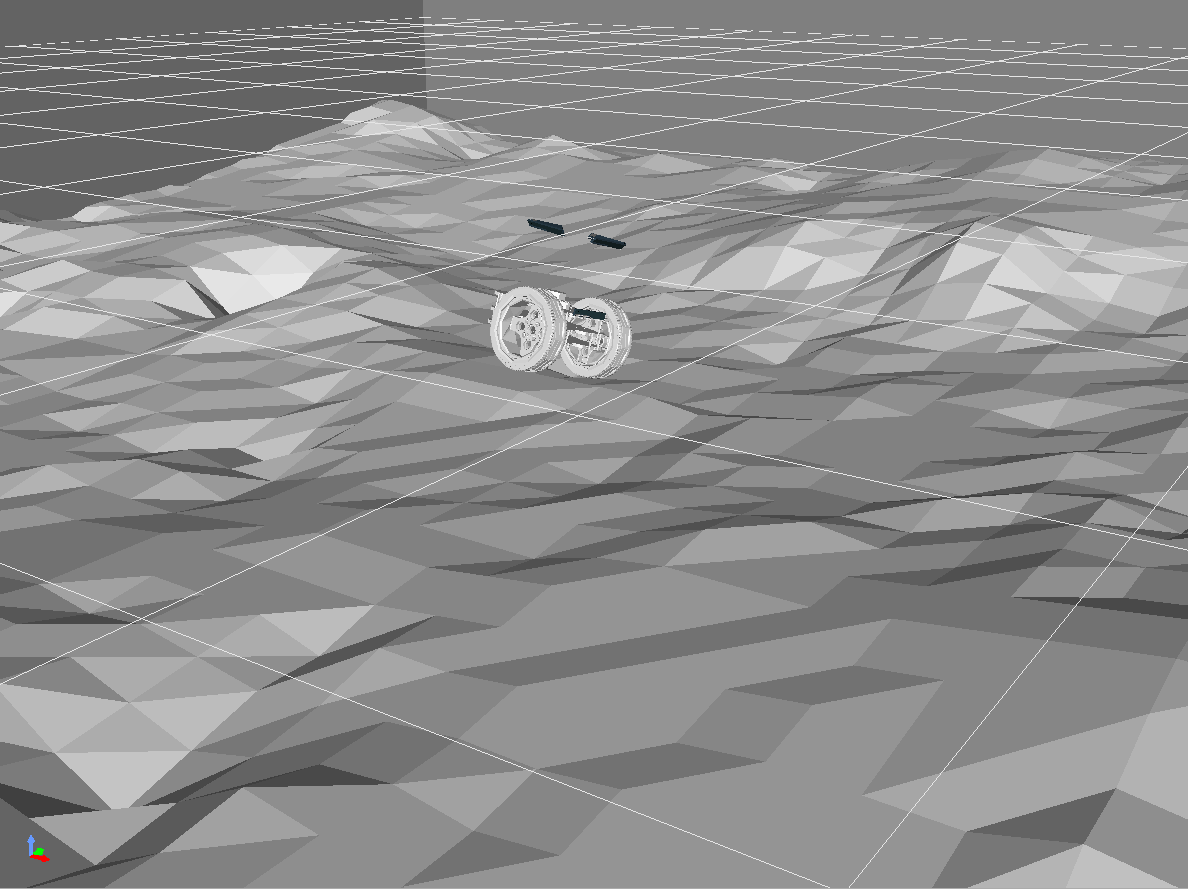
\includegraphics[keepaspectratio, scale=0.075]{figures/test_field_origin1.png}
  %   \subcaption{元の月面}\label{fig:field1}
  % \end{minipage}
  % \begin{minipage}[b]{0.45\linewidth}
  %   \centering
  %   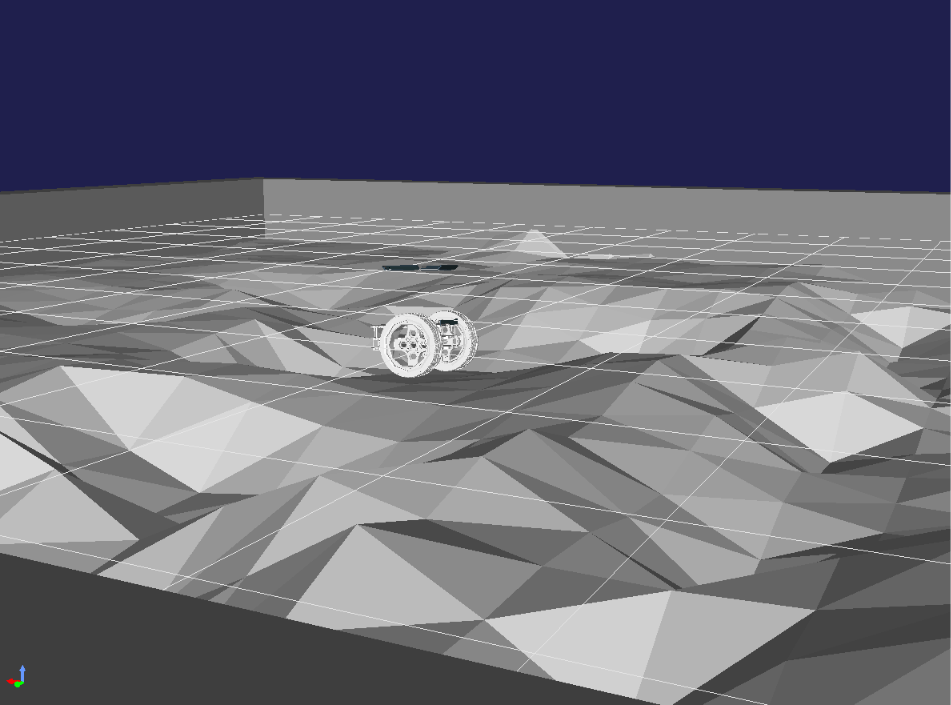
\includegraphics[keepaspectratio, scale=0.10]{figures/test_field1.png}
  %   \subcaption{生成した月面}\label{fig:field2}
  % \end{minipage}
  \begin{minipage}[b]{0.48\linewidth}
    \centering
    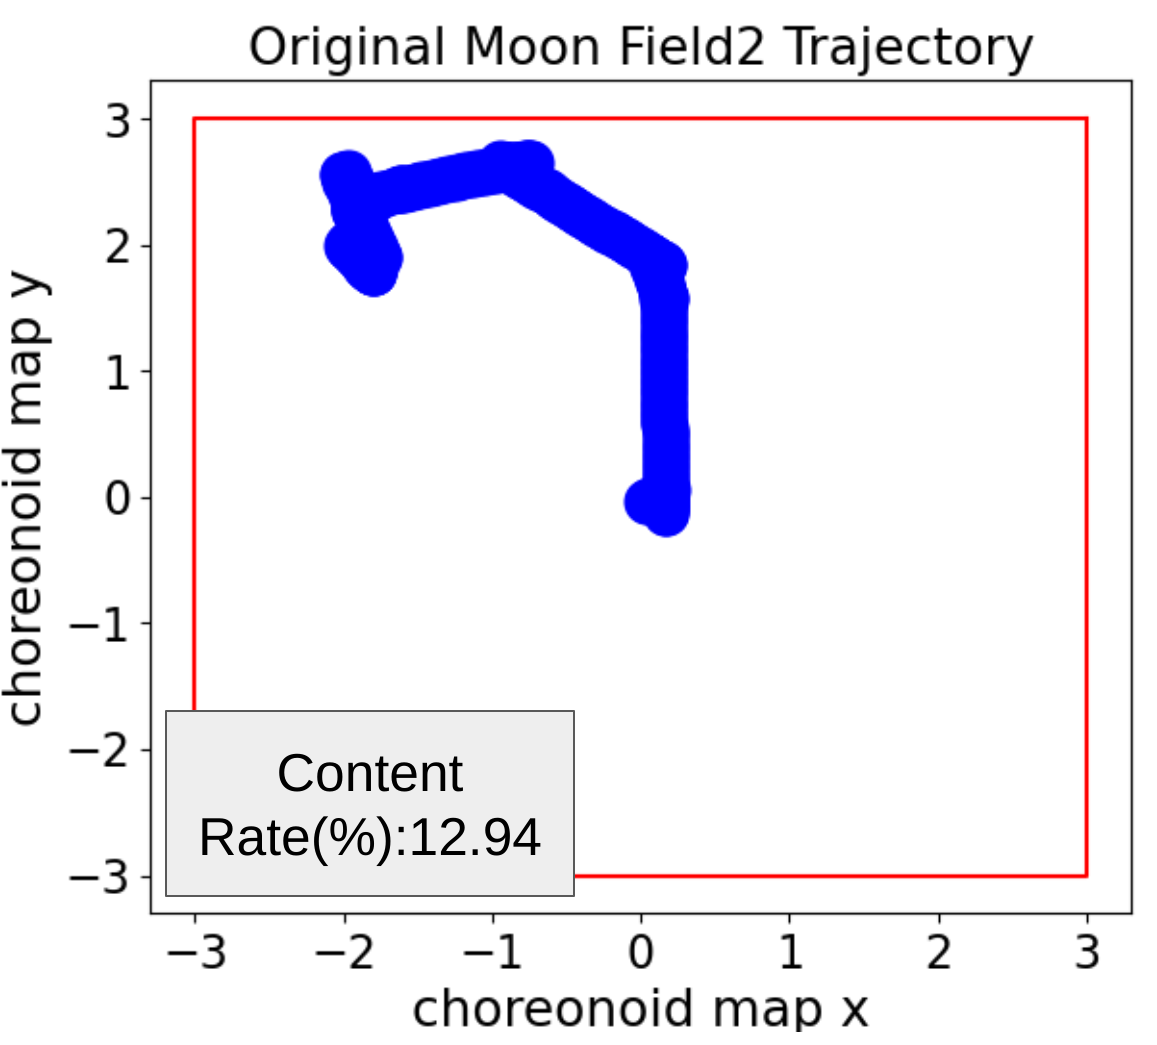
\includegraphics[keepaspectratio, scale=0.10]{figures/origin_moon_field2.png}
    \subcaption{元の月面の走行結果}\label{fig:result1}
  \end{minipage}
  \begin{minipage}[b]{0.48\linewidth}
    \centering
    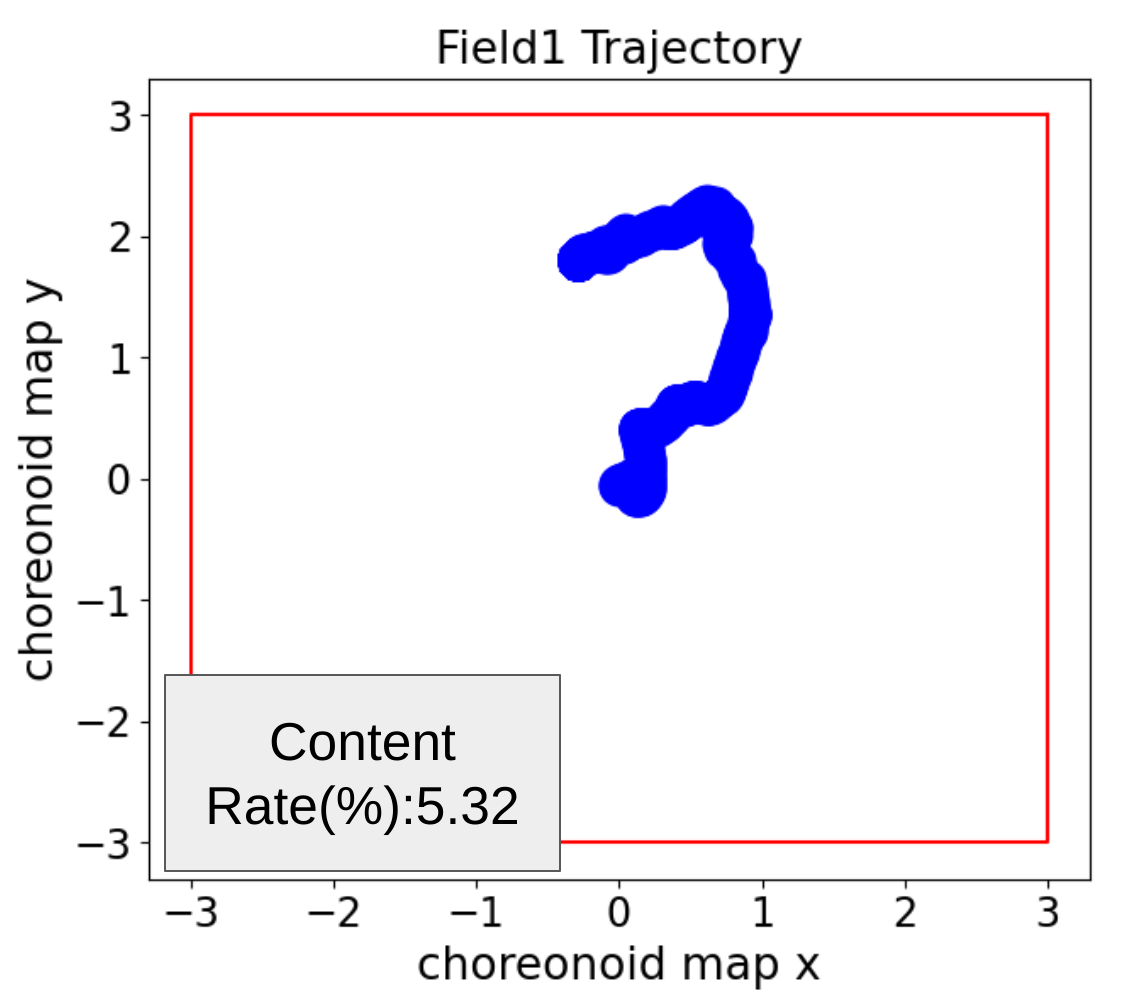
\includegraphics[keepaspectratio, scale=0.105]{figures/field1_trajectry.png}
    \subcaption{生成した月面の走行結果}\label{fig:result2}
  \end{minipage}
  \caption{実験結果}
\end{figure}

% \begin{table}[b]
%   \begin{center}
%     \begin{tabular}{|l|r|r|} \hline
%       Field & 含有率(%) \\ \hline
%       1 & 5.32 \\
%       2 & 56.20 \\ \hline
%     \end{tabular}
%   \end{center}
%   \caption{各フィールドに対する軌跡の含有率}\label{table:result}
% \end{table}

\section{おわりに}
本研究では3D-GANを用いて不整地を生成することで,走行計画に必要な学習用データを効率的かつ大規模に用意し,その走破性評価による実験フレームワークの作成を行った.これにより元の月面データの走破結果に近い生成地形を用いることで,少数の地形データで走行計画に必要な機械学習用データを効率的に収集できることが分かった.


%-----参考文献-----%

%%%  直書きスタイル %%%

% \begin{thebibliography}{9}
% 	\footnotesize
% 	\bibitem{bunken1}{	Goodwin, C.: Embodied Hearers and Speakers Constructing Talk and Action in Interaction,	Cognitive Studies, Vol.16, No.1, pp.51-64 (2009).}
% \end{thebibliography}
% \begin{thebibliography}{9}
% 	\footnotesize
% 	\bibitem{bunken1}{	Edward J. Smith, David Meger, Improved Adversarial Systems for 3D Object Generation and Reconstruction (2017).}
%   \bibitem{bunken1}{	清水 優, 高橋 友一, モデル化した不整地による評価フィールドを用いたレスキューロボットの動作・地図作成能力評価手法の提案 (2014).}
% \end{thebibliography}

%%%  bibtex使用スタイル %%%

\bibliographystyle{junsrt} %参考文献出力スタイル
\footnotesize\bibliography{references} %hoge.bibから拡張子を外した名前


\end{document}